Hybrid testing can help to reduce \textit{memory overhead} by 
limiting the number of states to an acceptable level. However, 
as mentioned in Section~\ref{sec:introduction}, symbolic pointers 
and loops will quickly generate lots of useless states that may 
not cover new code areas but bring serious performance overhead.

To address the large number of states forked from symbolic pointers, 
we propose a novel \textit{lazily concretization} of symbolic 
pointers which can not only reduce the number of states but also 
improve coverage. 
For symbolic loops, we introduce an optimization based on AFL's 
\textit{loop bucket} to control forking in symbolic loops. By 
doing this, execution can reach deeper code areas without 
generating lots of states. Both improvements will be discussed 
in the following sections.

\begin{figure}
\centering
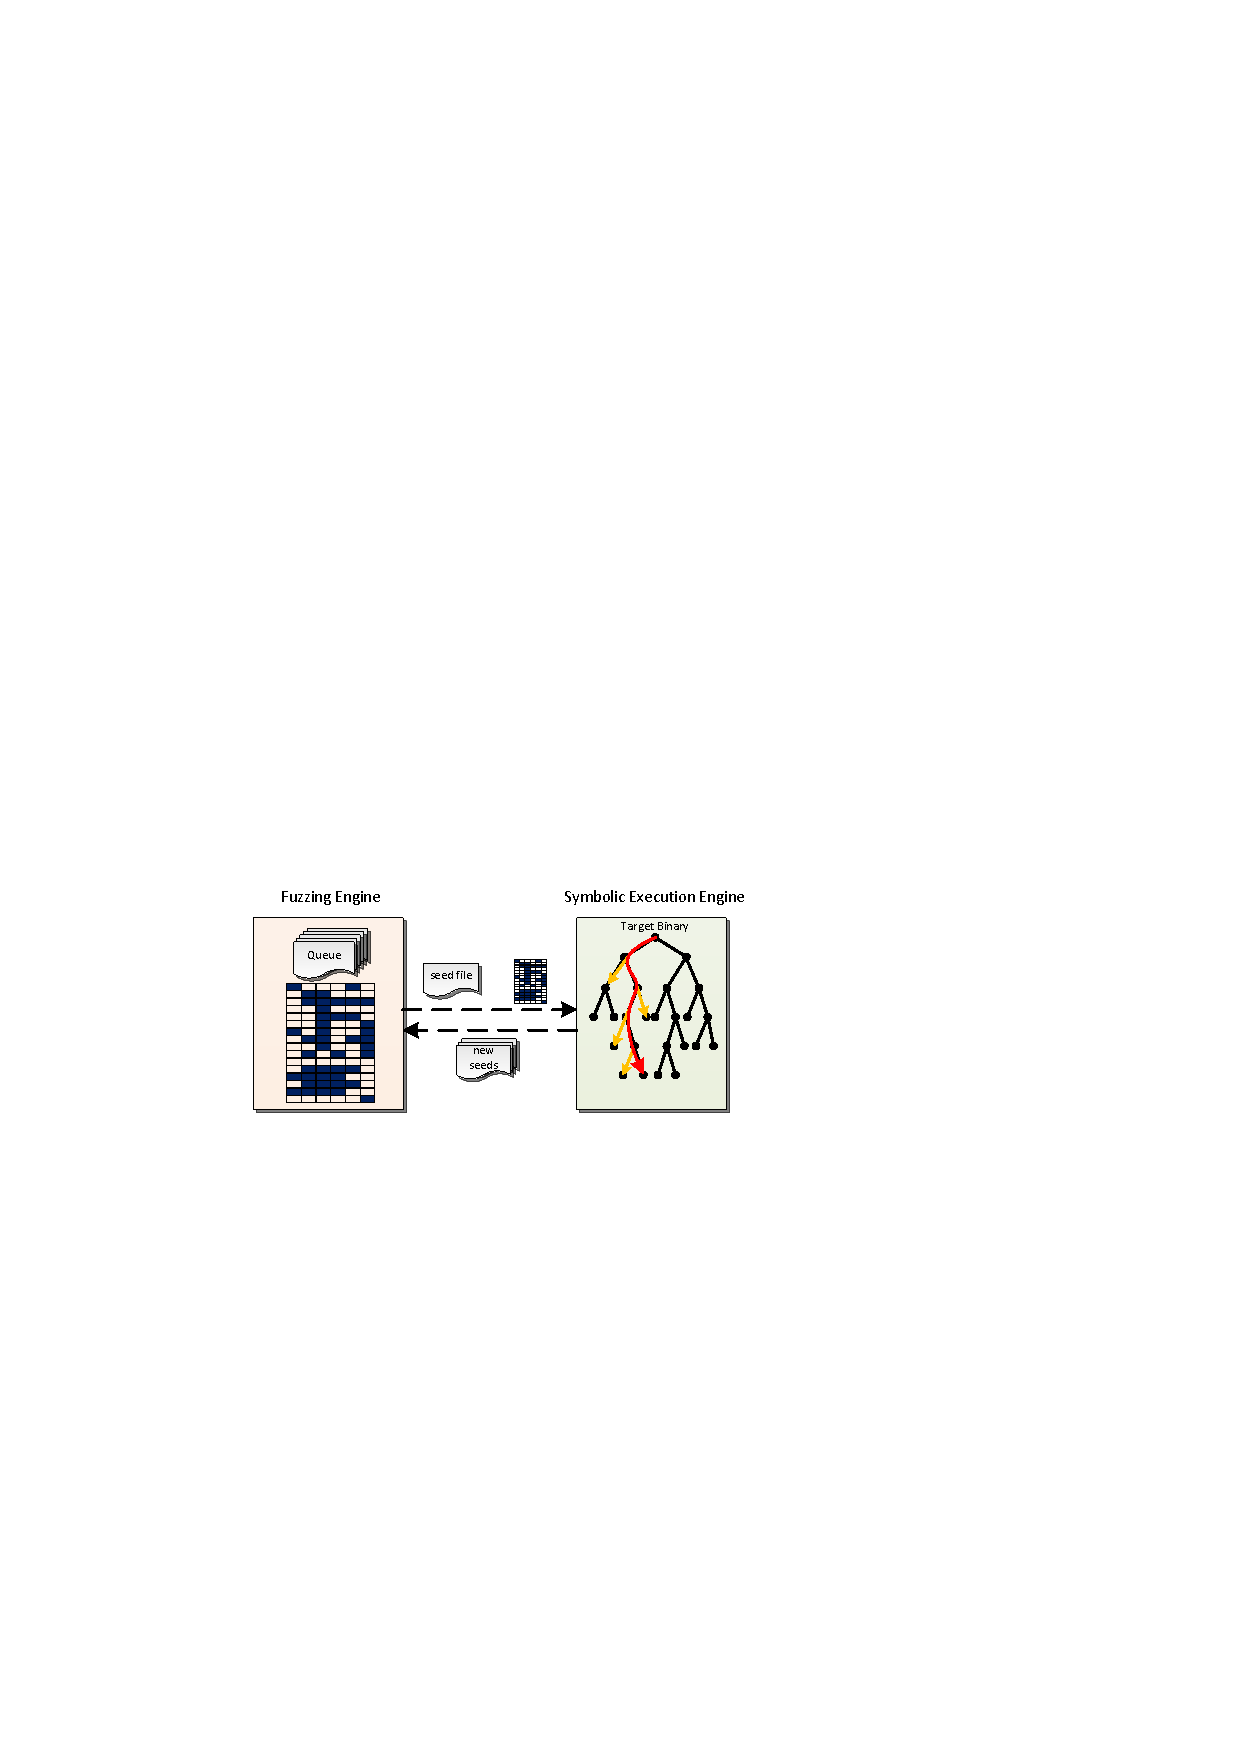
\includegraphics[width=0.5\textwidth]{figures/s2e-assist.pdf} 
\caption{Dynamic symbolic execution assisted fuzz testing. The 
	symbolic execution engine can help generate fresh seeds for 
	the fuzzing engine based on the seed files 	and the already 
	explored path information.}\label{s2e-assist}
\end{figure}

\subsection{Lazy Concretization of Symbolic Pointer}
The code snippet in Listing~\ref{RE-LCSP} shows the basic symbolic pointer 
problem in dynamic symbolic execution. The first parameter 
(i.e., \texttt{buf}) of function \texttt{looks\_ascii} points to memory 
that contains symbolic input data. The \texttt{nbytes} parameter is a 
concrete value that denotes the size of the memory buffer pointed by 
\texttt{buf}. \texttt{ubuf} is a shadow buffer which is used for further 
processing. 
Function \texttt{looks\_ascii} tries to determine whether each character 
of the symbolic input data appears in plain ASCII text, and returns 
immediately once a non-plain ASCII text character appears. 
The symbolic execution engine faces the symbolic pointer problem when executing 
the code at line 18 because \texttt{buf[i]} is from the symbolic input data. 
The memory range of \texttt{text\_chars[buf[i]]} spans from \texttt{\&text\_chars} 
to \texttt{\&text\_chars+255}. Since the binary executable loses the 
type information, the symbolic execution engine may need to explore all 256 possible
values for each \texttt{buf[i]} at the worst case. Meanwhile, the loop from line
17 to line 22 makes the trigger of the bug at line 26 even harder since more
states will be forked when \texttt{nbytes} is a larger one.
% Inaccurate expression for FSMM.
%Since \texttt{buf[i]} has 256 possible values (\textit{unsigned char}), 
%then the symbolic engine will fork state for each possible value (i.e., 
%fully symbolic memory model).
%This will cause the code at Line 18 to fork 
%$256^{nbytes}$ states, causing path explosion. The bug nested at line 26 
%will only be triggered when the states that satisfy the path condition 
%are scheduled for execution, which may never practically occur in the 
%face of path explosion. For example, suppose \texttt{nbytes} is 4, then 
%the worst case is that the bug can only be triggered after all 
%$256^4=4294967296$ states are scheduled.

There are different approaches for handling path explosion caused by
symbolic pointers. For example, treating memory address as \textbf{fully symbolic} 
enables the executor to reason about all possible values for symbolic pointer
\cite{song2008bitblaze, thakur2010directed, brumley2011bap, trtik2014symbolic}.
This can be achieved by either forking states or employing nested 
\textit{if-then-else} formulas which encode all possible values. 
However, since a symbolic address may pointer to any memory cell, fully symbolic
memory model fails to scale for real-world binary software. 
Some researches leverage the \textit{theories of arrays} to make fully symbolic 
memory model scalable \cite{cadar2006exe}\cite{cadar2008klee}. 
For example, KLEE \cite{cadar2008klee} forks states for values that reference 
different objects, and the \textit{theories of arrays} is leveraged within the same object.
However, since our target is to analyze binary executable whose object size of data structure is 
unavailable, the number of objects increases because each possible value may reference to a 
different object.
In contrast to reason about all possible values, a \textbf{partial symbolic} memory model has been proposed \cite{cha2012unleashing, avgerinos2014exploiting, Shoshitaishvili_firmalice-automatic}.  
The partial symbolic memory model tries to concretize all symbolic pointer write 
operation and treats symbolic pointer read operation using a fully 
symbolic memory model when contiguous interval of possible values is small enough.
However, if the possible values spans a large area, partial symbolic memory model
still needs to concretize the symbolic pointer which may lose some soundness paths.

%% Inaccurate description for fully and partial symbolic memory model.
%There are different approaches for handling path explosion caused by 
%symbolic pointers. For example, in the \textbf{fully symbolic memory model}, 
%each possible value of symbolic pointer will fork a corresponding state 
%\cite{song2008bitblaze, thakur2010directed, brumley2011bap, trtik2014symbolic}.
%In contrast, the \textit{address concretization} strategy will concretize 
%the pointer to a specific address \cite{godefroid2005dart, burnim2008heuristics}. 
%Obviously, the fully symbolic memory model may cause path explosion 
%(as mentioned before) and the address concretization may lose some 
%interesting paths. To mitigate the scalability problems of fully symbolic 
%memory model and the loss of interesting paths of address concretization, 
%a \textbf{partial symbolic memory model} has been proposed \cite{cha2012unleashing, avgerinos2014exploiting, Shoshitaishvili_firmalice-automatic}. The partial 
%symbolic memory model tries to concretize all symbolic pointer write 
%operation and treats all symbolic pointer read operation using a fully 
%symbolic memory model. However, because the instruction at line 18 is a 
%read operation, the partial symbolic memory model will still fork $256^{nbytes}$ states.

The \textit{lazy forking} strategy leveraged in S2E was proposed to avoid 
maintaining expensive symbolic pointers and ease the large number 
of states by forking \textit{pending states} in concolic 
execution \cite{chipounov2011s2e}. 
Consider a memory dereference instruction $I\in Inst$ in program $P$, 
suppose $I$ tries to access memory indexed by a symbolic expression 
$e_{addr}$.
Lazy forking treats such instruction $I$ as a conditional instruction 
and forks new states for $I$. It first evaluates the concrete value 
as $c_{addr}$, then it constructs an equal
expression $condition:= EQ(e_{addr}, c_{addr})$ 
which points $e_{addr}$ to this concrete value. Then it forks a 
new state $s_p=fork(s, ^\neg condition)$ which is labeled as a 
``pending state''. After that, each possible value of $e_{addr}$ 
will be exercised by systematically repeating this process. Even 
though lazy forking still needs to enumerate all possible values, 
it can avoid overhead by significantly reducing the total number 
of states that simultaneously exist in system. Here, 
the $condition$ is called a \textit{hard constraint} and 
$^\neg condition$ is called a \textit{soft constraint}.

For example, for the memory dereference instruction at line 18 
in Listing~\ref{RE-LCSP}, suppose the concrete value of 
\texttt{buf[i]} for $i\in[0,1,2,3]$ is `\texttt{A}'. 
In this case lazy forking will fork a new pending state and 
add the soft constraint $\texttt{buf[i]}\neq\texttt{`A'}$ to 
it. Meanwhile, the path constraint of the original state will 
be appended with the hard constraint $\texttt{buf[i]}=\texttt{`A'}$.
By doing this, the ``path explosion'' problem is postponed to a later moment.

However, the hard constraint may reduce the suffix feasible paths 
to a very small group. For example, suppose the address of a symbolic 
pointer can be expressed as $e_{addr}=f(v_1, v_2,\cdots, v_n)$, 
where $v_1, v_2,\cdots, v_n\in Var$ are variables of program $P$. 
Then expression $condition:= EQ(e_{addr}, c_{addr})$ will limit 
the current execution path only feasible when ($v_1, v_2,\cdots, v_n$) 
equals to ($c_1, c_2,\cdots, c_n$), where $c_i$ are the 
corresponding concrete values. 
Take the sample code in Listing~\ref{RE-LCSP}. The execution path 
to line 26 will be infeasible because the hard constraint limits 
the value of \texttt{buf[i]} ($i\in[0,1,2,3]$) to `\texttt{A}'. 
And the crash can only be triggered after enumerating all possible 
values for \texttt{buf[i]} ($i\in[0,1,2,3]$) in the worst case since
lazy forking still belongs to DFS state exploration strategy.
So even though lazy forking can ease the path explosion problem, 
it may still need to take longer time to trigger interesting paths. 
This will result in performance loss, because the symbolic 
execution engine will hold up the fuzzer. 

To mitigate this problem, we introduce a novel method 
\emph{lazy concretization of symbolic pointer} (LCSP) 
which is built on top of lazy forking. The detailed algorithm 
of LCSP is shown in Algorithm~\ref{LCSP}.


\lstinputlisting[label={RE-LCSP}, language=C,style=c,caption={A 
	motivating code derived from \texttt{file} in GNU Coreutils that contains symbolic pointer dereference at line 18.}, 
float=tp]{codes/real-eaxmple-LSP.c} 

Whenever the execution engine touches a symbolic pointer $e_{addr}$, it obtains 
the range of all possible values $\mathcal{R}$ by invoking function \texttt{getRange} 
in constraint solver. Then memory values $v$ within the range are dissolved
into buckets $\mathcal{B}=\langle v, addr\rangle$, where $v$ is the memory value; $addr$
is the set of memory cell's address whose memory value is $v$. 
After this, we reuse S2E's lazy forking method to pickup 
the buckets that contains the concrete value of this symbolic pointer.
For example, when executing the code at line 18 in Listing~\ref{RE-LCSP}, the range of 
the symbolic pointer is $\mathcal{R}=\texttt{\&text\_chars}+\{0, 1,\cdots, 255\}$.
By scanning the memory cells within $\mathcal{R}$, we can build 4 buckets, i.e., 

$\mathcal{B}_0=\{v=0| addr=[0,1,2,3,4,5,6,11,14,15,\cdots]\}$

$\mathcal{B}_1=\{v=1| addr=[7,8,9,10,12,13,\cdots]\}$

$\mathcal{B}_2=\{v=2| addr=[160,161\cdots, 253,254,255]\}$

$\mathcal{B}_3=\{v=3| addr=[128,129,130,\cdots,159]\}$

Since $e_{addr}$'s concrete value belongs to $\mathcal{B}_1$, we then
introduce a new symbolic variable $v_p$ into the engine and update current path constraint by adding expanded hard constraint $condition$ to it. 
$condition$ is descried as $P_\mathcal{B}\cap P_v\cap P_p$, where

$P_\mathcal{B}=\{\bigcup\limits_{i=0}^{Len_{addr}-1}e_{addr}=addr_i\}$;

$P_v=\{v_p=1\}$; 

$P_p=\{e_{addr}=\&\texttt{text\_chars}+0x41\}$.

During the following execution, all path conditions that related to the newly
introduced symbolic variable $v_p$ will be collected as pointer dereference constraint
$C_{pd}$.
This constraint is used to keep execution consistency.

\begin{algorithm}
 \LinesNumbered
  \caption{Lazy concretization of symbolic pointer}
  \label{LCSP}
  \KwIn{Current state $S$, pending states $S_P$, hard constraint $C_H$, 
  	    pointer dereference constraint $C_{pd}$.}
  \KwOut{Testcase $t_{lsp}$ if success.}
  $C_F = getFailedCondition()$\;
  % ignore cases that unrelated to symbolic pointer
  \If{$C_F$ \textbf{is not result from symbolic pointer}}
  {
  	return $null$\;
  }
  $offs = S.getInputOffset(C_F)$\;
  
  % Collect all possible bucket's addr to Solutions
  $extraCond\leftarrow True$\;
  \ForEach{$s_p$ in $S_P$}
  {
  	$off_{fork} = s_p$.getInputOffset($s_p$.forkCondition)\;
  	\If{$off_{fork}$ not in $offs$}
  	{continue\;}
  	$\mathcal{B}=s_p$.buckets\;
  	$e_{addr} = s_p$.getForkAddr()\;
  	% find all satisfied buckets
  	$\mathcal{B}_{sat}=s_p$.getSATBuckets($C_{pd}$, $\mathcal{B}$)\;
  	
  	% sieve real solutions out
  	$curExtraCond\leftarrow False$\;
  	\ForEach{$addr$ in $\mathcal{B}_{sat}$.addr}
  	{
      $s_{tmp} = S$.clone()\;
      $s_{tmp}$.getConditions().strip($C_H$)\;
      $s_{tmp}$.addConstraint($C_F$)\;
      $C_{new}\leftarrow \{e_{addr}=addr\}$\;
      $success = s_{tmp}$.evaluate($C_{new}$)\;
      \If{success}
      {$curExtraCond\leftarrow curExtraCond\cup C_{new}$\;}
  	}
  	$extraCond\leftarrow extraCond\cap curExtraCond$\;
  }
  
  $s_{tmp} = S$.clone()\;
  $s_{tmp}$.getConditions().strip($C_H$)\;
  $s_{tmp}$.getConditions().strip($C_{pd}$)\;
  $s_{tmp}$.addConstraint($extraCond$)\;
  
  $(success, t_{lsp}) = s_{tmp}$.generateTestcase()\;
  \If{$success$}
  {
    return $t_{lsp}$;
  }
  return $null$\;
\end{algorithm}

When performing lazy forking, all the states whose path constraints 
contain the soft constraints will be collected into \emph{Pending States}
as well as the buckets. 
These pending states are grouped by the program variables (e.g., each 
byte in an input file) that affect the corresponding soft constraint. 
They are also ordered along with the execution trace.
Then when the dynamic symbolic execution engine detects an infeasible 
branch due to hard constraints from symbolic pointer (line 3$\sim$5), 
the branch condition $C_F$ will be 
investigated to extract the program variables $offs$ (line 5).



Since we introduce new symbolic variable when dereferencing a symbolic pointer,
we need to make sure all conditions in $C_{pd}$ are satisfied so that the generated
test case can keep execution consistency.
Line 14 collects all satisfied buckets into $\mathcal{B}_{sat}$. The collect procedure
is light-weight since \texttt{getSATBuckets} only needs to evaluate $C_{pd}$
under each bucket's key (i.e.,$v$).
For each satisfied bucket, real solutions for current $e_{addr}$ are sieved out 
(line 16$\sim$25). This is achieved by evaluating each $addr$ in $\mathcal{B}_{sat}$
(line 20\&21). All $C_{new}$ evaluated as True will be collected together (line 22
$\sim$24). The $\cup$ in line 23 compact consecutive $addr$s into a range expression.
For example, $\{e_addr=4\}$, $\{e_addr=5\}$ and $\{e_addr=6\}$ will be transformed to
$\{4<=e_addr<=6\}$.

By analyzing all pending states, the final extra condition $extraCond$ is constructed
(line 26).
After this, we remove $C_H$ and $C_{pd}$ from a newly cloned state $s_{tmp}$
from current state and append
the final extra condition to it (line 29$\sim$31). 
The reason why $C_{pd}$ is stripped is because it is already satisfied at line 14.
After appending all related conditions, the dynamic symbolic execution 
engine will try to generate a new test case (line 32), and once the 
generation successes, the test case $t_{lsp}$ will be sent to the 
fuzzer to find more paths.

For the code in Listing~\ref{RE-LCSP}, suppose \texttt{nbytes} is 5. 
Then when dynamic symbolic execution reaches line 24, there will be 
six states in the system: one execution state $S_0$ and five pending 
states ($P_0$, $P_1$, $P_2$, $P_3$, and $P_4$). $P_i$ is forked when 
dereferencing \texttt{buf[$i$]} at line 18. And pointer dereference
constraint $C_{pd}$ is $\{v_0=T\cap v_1=T\cap v_2=T\cap v_3=T\cap v_4=T\}$,
where $v_i$ is introduced for each symbolic pointer dereference at
line 18.

Because of the hard constraint, the four condition instructions at line 24
is infeasible. 
For example, for condition \texttt{ubuf[0]==`D'}, since line
18 introduces $\texttt{buf[0]=`A'}$, condition \texttt{ubuf[0]==`D'} cannot
be satisfied. LCSP first checks the input offset that results in this infeasible
condition and deals all pending states related to this offset. Based on this,
only $P_0$ is analyzed in order to break \texttt{ubuf[0]==`D'}. As mentioned before,
there are four buckets for $P_0$, i.e., $\mathcal{B}_0$, $\mathcal{B}_1$, $\mathcal{B}_2$,
$\mathcal{B}_3$. Then \texttt{getSATBuckets} verifies keys for all these four buckets 
to sieve the feasible ones. In this example, $\mathcal{B}_{sat}=\{\mathcal{B}_1\}$ since
$v_0=T$ in $C_{pd}$ must be satisfied. 

Then from line 16 to line 25 in Algorithm~\ref{LCSP} evaluates each $addr$ in $\mathcal{B}_1$ to build the final extra condition. The final constructed extra
condition for \texttt{ubuf[0]==`D'} in this example is $extraCond=\{\texttt{buf[0]=`D'}\}$.
This $extraCond$ keeps not only $C_F$ but also $C_{pd}$ be satisfied.
Then LCSP fixes current path condition by stripping unrelated conditions and adding
$\{\texttt{buf[0]=`D'}\}$ to it. After this, it invokes constraint solver to 
generate a fresh test case. Here, after breaking condition \texttt{ubuf[0]==`D'}, the 
generated test case is \texttt{DAAAA}. This test case will be sent to the fuzzer and the
remained three conditions at line 24 will be solved in the same way. Thus, based on this algorithm, we can generate at least one fresh test case 
that satisfies the branch condition whenever a branch is infeasible 
because of lazy forking. 

%Then path constraint for each states is shown in Table~\ref{table:path-conditions}.
%
%\begin{table}[!b]
%\processtable{Path Constraint for each state when reaching line 24 in Listing~\ref{RE-LCSP}.
%	\label{table:path-conditions}}
%{\begin{tabular*}{20pc}{@{\extracolsep{\fill}}lccccc@{}}\toprule
%State  & buf[0] & buf[1] & buf[2] & buf[3] & buf[4]\\ 
%\midrule
%		$S_0$  &  $=$ `A' & $=$ `A' & $=$ `A' & $=$ `A' & $=$ `A' \\
%		$P_0$  &  $\neq$ `A' & N/A & N/A & N/A & N/A \\
%		$P_1$  &  $=$ `A' & $\neq$ `A' & N/A & N/A & N/A\\
%		$P_2$  &  $=$ `A' & $=$ `A' & $\neq$ `A' & N/A & N/A \\
%		$P_3$  &  $=$ `A' & $=$ `A' & $=$ `A' & $\neq$ `A' & N/A \\
%		$P_4$  &  $=$ `A' & $=$ `A' & $=$ `A' & $=$ `A' & $\neq$ `A' \\
%\botrule
%\end{tabular*}}{}
%\end{table}
%
%The hard constraint for $S_0$ is $C_{H}\leftarrow$ \{\texttt{buf[0]$=$`A'\& buf[1]$=$`A'\&buf[2]$=$`A'\&buf[3]$=$`A'\&buf[4]$=$`A'}\}. 
%Because of $C_{H}$, the branch condition at line 24\&25 ($C_{F}\leftarrow$ \{\texttt{buf[0]$=$`D'\&buf[1]$=$`E'\&buf[2]$=$`A'\&buf[3]$=$`D'}\}) will 
%be infeasible.
%Based on \textit{LCSP}, the path conditions of $S_0$ (except for the related 
%hard conditions) will be append to each pending state to generate new test case. 
%After stripping the related hard conditions, the \textit{Conditions} at line 
%6 in Listing~\ref{LCSP} will be $\texttt{buf[4]}=\texttt{`A'}$. 
%Then \textit{Conditions} will be added to each pending state. For example, 
%the path constraint of $P_0$ after adding such conditions will be 
%\{\texttt{buf[0]$\neq$`A' \& buf[4]$=$`A' \& buf[0]$=$`D' \& buf[1]$=$`E' \& buf[2]$=$`A' \& buf[3]$=$`D'}\}. After solving this path constraint, we can successfully 
%generate a test case that satisfies the condition at line 24\&25 and 
%triggers the bug at line 26. 
%
%An interesting point in our example is that $P_1$, $P_2$, $P_3$, and 
%$P_4$ cannot successfully trigger this bug. This does not mean that 
%these states are useless. 
%For example, if the condition at line 24\&25 is 
%\{\texttt{buf[0]$=$`A' \& buf[1]$=$`B' \& buf[2]$=$`C' \& buf[3]$=$`D'}\}, 
%then $P_1$ can successfully generate a corresponding test case 
%that triggers the bug.


%% Remove this proof since the consistency is kept by the constraint solver.
%But we still need to prove this test case 
%will steer the program to execute the same path with the original 
%state and then covers the branch that fails in the original state. 
%A quick execution consistency proof is explained as follows:
%
%Let $P_A$ be the execution path of a state $A$ which contains 
%the following branches:
%\begin{center}
%$P_A:(B_0) \rightarrow (B_1) \rightarrow (B_2) \rightarrow 
%(B_3) \rightarrow (B_4) \rightarrow (B_5) \rightarrow (B_6) \rightarrow (B_u)$
%\end{center}
%
%\noindent where $B_i$ refers to the $i$-th branch, and $B_u$ 
%denotes the infeasible branch that because of the extra hard constraint.
%And its path constraint is:
%\begin{center}
%$PC_A\leftarrow \displaystyle \bigcap\limits_{i=0}^{6} CB_i \cap CB_u$
%\end{center}
%, where the $CB_i$ denotes the path condition at branch $B_i$.
%
%Assume that the hard constraint is $var=0xAB$ which is originated 
%from lazy forking from $B_1$. 
%We also assume that the branch conditions at $B_3$ and $B_5$ are 
%also affected by $var$; state $B$ is the corresponding pending state 
%forked from $B_1$, and its path constraint is:
%\begin{center}
%$PC_B\leftarrow\displaystyle CB_0 \cap ^\neg CB_1$
%\end{center}
%, where $^\neg CB_1$ is the soft constraint.
%
%Then, according to the \textit{LCSP} algorithm in Listing~\ref{LCSP}, 
%when state $A$ detects the infeasible branch $B_u$ because of hard 
%constrain, all the related constraints except the hard constraint 
%of state $A$ will be added to state $B$. After that, the path 
%constraint of state $B$ will be:
%
%\begin{center}
%$PC_B\leftarrow\displaystyle CB_0 \cap ^\neg CB_1 
%\cap (\bigcap\limits_{i=0,i \neq 1}^{6} CB_i) \cap ^\neg CB_u$
%\end{center}
%where $^\neg CB_u $ is the branch condition we want to cover 
%and $\bigcap_{i=0,i \neq 1}^{6} CB_i$ is the conditions from 
%state $A$ after stripping the hard constraint.
%
%We need to prove the following formula:
%
%\begin{center}
%$\mathbb{Z}=\{var\arrowvert PC_B(var) = True\} \neq \emptyset$
%\end{center}
%
%As there are only two branches before $B_u$ that depend on $var$, 
%the expression $PC_B$ can be simplified to:
%\begin{center}
%$PC_B\leftarrow^\neg CB_u \cap ^\neg CB_1 \cap CB_3 \cap CB_5$
%\end{center}
%
%There are two possible cases for $CB_3 \cap CB_5$:
%\begin{center}
%case1: $CB_3 \cap CB_5 = (var = 0xAB)$
%
%case2: $CB_3 \cap CB_5 \neq (var = 0xAB)$
%\end{center}
%
%Under the first case, the path to $B_u$ is only feasible when 
%$var$ equals to $0xAB$. So the edge $^\neg B_u$ can never be 
%satisfied (i.e., \emph{dead code}) because $(var = 0xAB) \subseteq CB_u$. 
%For the second case, there must be at least one feasible solution 
%for $var$ that satisfies the soft constraint $^\neg CB_1$, so 
%$^\neg CB_1 \cap \bigcap_{i=0,i \neq 1}^{6} CB_i$ can be evaluated 
%to $True$ for some specified values of $var$. This has proved that 
%there must be at least one test case under $PC_B$ that can steer 
%the program to the infeasible branch $B_u$.
%
%Similarly, for branch condition $B_u$, there are also two possible cases:
%\begin{center}
%case1: $\displaystyle ^\neg CB_1 \cap \bigcap\limits_{i=0,i\neq 1}^6 CB_i \subseteq CB_u$
%
%case2: $\displaystyle ^\neg CB_1 \cap \bigcap\limits_{i=0,i\neq 1}^6 CB_i \nsubseteq CB_u$
%\end{center}
%
%The first case, which can also be expressed as 
%$^\neg CB_u \cap ^\neg CB_1 \cap \bigcap_{i=0,i\neq 1}^6 CB_i = \emptyset$, 
%is the case of \emph{dead code}. And the second case can be transformed into:
%\begin{center}
%$\displaystyle ^\neg CB_u \cap ^\neg CB_1 \cap \bigcap\limits_{i=0,i\neq 1}^6 CB_i \neq \emptyset \implies \mathbb{Z} = \{var\arrowvert PC_B(var) = True\} \neq \emptyset$
%\end{center}
%
%\noindent which means there must be at least one feasible value 
%that satisfies the false branch of $B_u$.
%
%So above all, we can draw a conclusion that our \emph{LCSP} algorithm 
%can keep the execution consistency when $^\neg B_u$ is not dead code.

\subsection{Optimization for Symbolic Loop}
Symbolic loop, whose loop control variable depends on symbolic data, 
is another common cause of path explosion since its loop times may 
range from 0 to infinite theoretically. 
Even though the hybrid testing method can ease path explosion, the 
states forked from a symbolic loop will quickly force the number of 
states to increase to the budget's upper bound. 

\lstinputlisting[label={RE-SLB}, language=C,style=c,caption={A motivating 
	example to demonstrate path explosion raised by symbolic loops.}]
{codes/example-SLB.c} 

The code snippet in Listing~\ref{RE-SLB} demonstrates this problem. 
Function \texttt{verify\_packet} reads the \texttt{length} of the 
raw data from the \texttt{packet} at line 4.
 Then from Line 6 to 10, it investigates each bytes in the raw data 
 to determine whether there exists the ending descriptor 
 (i.e., \texttt{0xFF}) through a loop structure. 
 Suppose we have a test case from the seed queue of 
 the fuzzer and its \texttt{length} is \texttt{0xAA}, 
 then the symbolic loop 
 from line 6 to 10 (\texttt{length} is symbolic) 
 will result in path explosion.
 Because the possible value of \texttt{length} is in the 
 range of [0, $2^{32}-1$], $2^{32}$ states will be forked from 
 line 6 in the worst case. 
Most of the forked states from line 6 may not contribute 
to any new code coverage but only bring performance overhead.
It is therefore important to also handle symbolic loops. 

A \textit{boundary state prioritization} method has been proposed 
to ease the path explosion problem due to symbolic loops.
The key idea of this prioritization is to defer the analysis of 
uninteresting states based on the likelihood of a security vulnerability \cite{cab-fuzz}. 
Specifically, it focuses only on three types of states for a symbolic 
loop: \textit{no loop execution}, \textit{single loop execution}, and 
\textit{the largest number of loop executions}.
The author implemented such a strategy within S2E \cite{chipounov2011s2e} 
and produced a vulnerability detection tool \textit{CAB-Fuzz}.
It successfully found 21 undisclosed unique crashes in Windows 7 and 
Windows Server 2008 \cite{cab-fuzz}.
 
We extend this boundary state prioritization method by integrating it 
with the \emph{Loop Bucket} mechanism employed in AFL \cite{online:afl} 
to achieve better performance on finding vulnerabilities.
AFL utilizes \emph{Loop Bucket} to avoid collecting too many test cases 
which only affect the loop times into the seed queue \cite{online:afl}. 
It groups the loop times into 8 different buckets, i.e., 
[1, 2, 3, 4-7, 8-15, 16-31, 32-127, 128+]. Only changes that occur 
between different buckets will be regarded as new behaviors. 
Based on this idea, we proposed a \textit{Symbolic Loop Bucket} (SLB) 
to handle the symbolic loop when performing hybrid testing. The 
algorithm of SLB is described in Algorithm~\ref{SLB}.

Loops are extracted from the target program by static analysis. 
These loops will be configured in the dynamic symbolic execution 
engine to help it recognize loops in runtime. All the symbolic loops 
can be distinguished from the others by checking whether the loop 
exit condition is affected by symbolic data or not (line 1$\sim$3). 
For the edge belongs to symbolic loop, the uncovered loop buckets 
for this loop will be obtained by analyzing the \textit{Bitmap} 
mentioned before (line 5). 
In already covered loop buckets, the program will loop for one more 
time without forking new state (line 16\&17). Once an uncovered bucket 
is reached, the corresponding test case will be generated and then 
this uncovered bucket will be removed from the uncovered loop buckets 
to avoid generating multiple test cases (line 7$\sim$12). After 
generating test cases for all the uncovered buckets, the loop will 
be prohibited from being executed for more times. This can make sure 
that all the loop buckets will be covered without causing path explosion.

\begin{algorithm}
  \LinesNumbered
  \caption{Symbolic loop bucket.}
  \label{SLB}
  \KwIn{Configured Loops $L$, Current Edge $CE$ and Bitmap $B_p$}
  \KwOut{Generated test cases $t_{slb}$}  
  \If{not $IsaLoopCycleEdge(L,CE)$ or not $IsaSymLoop(CE)$}
  {
    return;
  }
  $loopTimes$ = 1\;
  $UBs$ = $ParseUncoveredBuckets(B_p)$\;
  \While{TRUE}
  {
    \ForEach{$ub$ in $UBs$}
    {
      \If{$loopTimes$ within $ub$}
      {
        $t_{slb}.add(GenerateTestcase())$\;
        $UBs$.$remove(ub)$\;
      }
    }
    \eIf{$UBs$ is $null$}
    {
      return $t_{lsb}$\;
    }{
      $ExecuteOneCycle()$\;
      $loopTimes += 1$\;
    }
  }
\end{algorithm}  

For the symbolic loop in Listing~\ref{RE-SLB}. Suppose previous 
test cases have covered the buckets of [1], [2], [3], and [4-7]. 
Then \textit{UBs} at line 5 in Algorithm~\ref{SLB} will consist of 
[8-15], [16-31], [32-127], and [128+]. 
$\textit{loopTimes}=[1, 2, \cdots, 7]$ will not fork any new states 
according to line 15 to 18. Then once the \textit{loopTimes} reaches 
8 which belongs to an uncovered bucket [8-15], the engine forks a 
new state,  generates the corresponding the test case, and removes 
bucket [8-15] from \textit{UBs}. The execution engines will not 
fork new states until \textit{loopTimes} reaches 16, 32 and 128. 
Once all the loop buckets are covered, the forking in this 
symbolic loop will be disabled. It will continue cycling until 
\textit{loopTimes} reaches the concrete value of \texttt{length} 
(i.e., \texttt{0xAA}) and then exercise deeper code areas.
